\documentclass{beamer}
\usetheme[white]{Wisconsin}
\usepackage{longtable}
\usepackage{graphicx}
\usepackage{listings}
\usepackage{color}
%% The amssymb package provides various useful mathematical symbols
\usepackage{amssymb}
%% The amsthm package provides extended theorem environments
\usepackage{amsthm} \usepackage{amsmath}
%% \usepackage{eqnarray}
\usepackage[mathcal]{euscript} \usepackage{color}
\usepackage{textcomp}
\usepackage{algorithm,algorithmic}
\usepackage[retainorgcmds]{IEEEtrantools}
\usepackage[absolute,overlay]{textpos}
  \setlength{\TPHorizModule}{1mm}
  \setlength{\TPVertModule}{1mm}
\definecolor{listinggray}{gray}{0.9}
\definecolor{lbcolor}{rgb}{0.9,0.9,0.9}
\lstset{
  backgroundcolor=\color{lbcolor},
  tabsize=4,
  rulecolor=,
  language=c++,
  basicstyle=\scriptsize,
  upquote=true,
  aboveskip={1.5\baselineskip},
  columns=fixed,
  showstringspaces=false,
  extendedchars=true,
  breaklines=true,
  prebreak =
  \raisebox{0ex}[0ex][0ex]{\ensuremath{\hookleftarrow}},
  frame=single,
  showtabs=false,
  showspaces=false,
  showstringspaces=false,
  identifierstyle=\ttfamily,
  keywordstyle=\color[rgb]{0,0,1},
  commentstyle=\color[rgb]{0.133,0.545,0.133},
  stringstyle=\color[rgb]{0.627,0.126,0.941},
}

%% colors
\setbeamercolor{boxheadcolor}{fg=white,bg=UWRed}
\setbeamercolor{boxbodycolor}{fg=black,bg=white}

%%----------------------------------------------------------------------------%%
\author{Luke J. Kersting
    \\ NEEP
    \\ University of Wisconsin - Madison
    \\ SNL Meeting
}

\date{\today}
\title{Electron Mode in FRENSIE}
\begin{document}
\maketitle

%%----------------------------------------------------------------------------%%
\begin{frame}{Electron Transport in FRENSIE}

  \begin{block}{Forward Mode}
    \begin{itemize}
      \item Condensed History
      \item Secondary Particles
      \item Atomic Relaxation
      \item Simulation of hard electron transport events
      \begin{itemize}
         \item Atomic excitation
         \item Hard elastic scattering
         \item Electroionization
         \item Bremsstrahlung
      \end{itemize}
    \end{itemize}
  \end{block}
    
  \begin{block}{Adjoint Mode}
    \begin{itemize}
      \item Hybrid Multigroup/Continuous-Energy Monte Carlo using Boltzmann-Fokker-Planck Equation (BFP)
      \item Other Possible Adjoint Methods
    \end{itemize}    
  \end{block}  

\end{frame}


%%----------------------------------------------------------------------------%%
\begin{frame}{Electron Transport in Monte Carlo Codes}

  \begin{block}{MCNP}
    \begin{itemize}
      \item Historically has only used a condensed-history approached with Goudsmit-Saunderson multiple scattering techniques.
      \item MCNP6 implemented a single-event method for energies below 1 keV, 
              were the condensed-history method no longer holds.
    \end{itemize}
  \end{block}
    
  \begin{block}{Penelope}
    \begin{itemize}
      \item Implements a mixed method that simulates soft (condensed-history) 
              events below a cutoff energy/angle and hard (single-events) above.
    \end{itemize}    
  \end{block}

  \begin{block}{EGS}
    \begin{itemize}
      \item Condensed History Method
      \item Historically used Moli\`ere Multiple Scattering Theory
      \item EGS5 implemented Goudsmit-Saunderson Multiple Scattering to take into account spin and relativistic effects needed in the MeV range
    \end{itemize}    
  \end{block}
    

\end{frame}


%%----------------------------------------------------------------------------%%
\begin{frame}{Electron Mode}

  \begin{block}{FRENSIE}
    \begin{itemize}
      \item Hard events implemented using cross-sectional data from ACE Tables
      \item Condensed history method will be chosen in conjunction with an adjoint method
      \item Ultimately hope to implement a mixed method for forward transport
    \end{itemize}    
  \end{block}
  
  \begin{block}{Current Capabilities}
    \begin{itemize}
      \item Single Scattering Events from 100 GeV to 10 eV
      \item Elastic, Bremsstrahlung, Electroionization, Atomic Excitation 
      \item Secondary particles created, but photons not tracked
      \item Atomic relaxation implemented
    \end{itemize}
  \end{block}
    
  \begin{block}{Known Issues}
    \begin{itemize}
      \item Absorption at low energies
      \item Negative energy from Electroionization
    \end{itemize}    
  \end{block}  

\end{frame}

%%----------------------------------------------------------------------------%%
\begin{frame}{Atomic Excitation}

  \begin{block}{Reaction}
    \begin{itemize}
      \item There is no angular deflection.
      \item There are no secondary particles.
      \item Only energy loss needs to be taken into account
    \end{itemize}
  \end{block}  

~~\\
  \begin{block}{Implementation}
    \begin{itemize}
      \item Energy dependent electron energy loss are tabulated in ACE tables.
      \item No sampling is required for this process.   
    \end{itemize}
  \end{block}  

\end{frame}

%%----------------------------------------------------------------------------%%
\begin{frame}{Hard Elastic Scattering}
  
  \begin{block}{Reaction}
    \begin{itemize}
      \item There is no energy loss.
      \item There are no secondary particles.
      \item Only angular deflection needs to be taken into account.
    \end{itemize}
  \end{block}  
      
  \begin{block}{Implementation}
    \begin{itemize}
      \item ACE tables provide histogram CDF of the outgoing angle cosine, \textmu, 
            for $14-16$ energy groups.
      \item for $\mu > 0.999999$ an analytical function, $f(\mu)$, derived from Moli\`ere's screening factor is used to compute the scattering angle.
    \end{itemize}

  \begin{equation*}
    f(\mu) = \frac{A}{(\eta + 1 - \mu)^2}
  \end{equation*}

  \begin{equation*}
    \eta(E,Z) = \frac{1}{4}\left(\frac{\alpha mc}{0.885p}\right)^2 Z^{2/3}[1.13+3.76(\alpha Z/\beta)^2]
  \end{equation*}
  
    \end{block}  


\end{frame}

%%----------------------------------------------------------------------------%%
\begin{frame}{Electroionization}

  \begin{block}{Reaction}
    \begin{itemize}
      \item The subshell is directly sampled.
      \item A knock-on electron is ejected.
      \item The incident electron energy is reduced by the $E_{knock} + E_{binding}$.
      \item Conservation of momentum is used to find the scattering and ejection angles.
      \end{itemize}
  \end{block}  
      
  \begin{block}{Implementation}
    \begin{itemize}
      \item ACE tables provide CDF of the knock-on energy, $E_{knock}$, based on the incident electron energy.
      \item The scattering and ejection angles are sampled independently breaking from a purely analog sampling.
      \item The shell vacancy is handled using atomic relaxation data. 
    \end{itemize}
  \end{block}  

\end{frame}

%%----------------------------------------------------------------------------%%
\begin{frame}{Electroionization Scattering Angle}

{\large Conservation of Momentum}
  \begin{align}
    (p_{knock}c = & (pc)^2 + (p'c)^2 - 2pp'cos(\theta) \nonumber \\
   cos(\theta) = & \frac{(pc)^2 + (p'c)^2 - (p_{knock}c)^2}{2pp'}  \nonumber
  \end{align}

{\large Conservation of Energy}
  \begin{equation*}
    (E + m_c^2) + (m_c^2) =(E' + m_c^2) + (E_{knock} + m_c^2) + E_{Binding}
  \end{equation*}
Assume the binding energy is negligible 
  \begin{equation*}
    E = E' + E_{knock}
  \end{equation*}
  Solving independently you obtain:
  $$ cos(\theta) = \frac{E'}{E}\frac{p}{p'}~~~~\text{and}~~~~
  cos(\phi)=\frac{E_{knock}}{E}\frac{p}{p_{knock}}$$


\end{frame}

%%----------------------------------------------------------------------------%%
\begin{frame}{Sampling Electroionization}
  
{\large The original sampling routine implemented in FRENSIE sampled negative electrons energies. } \\ 
~~\\

  \begin{itemize}
    \item ACE tables provide CDF of the knock-on energy, $E_{knock}$, based on the incident electron energy.
    \item The original implementation randomly selected whether to sample the upper or lower energy bin.
    \item A correlated sample must be made to avoid non physical values.
  \end{itemize}

\end{frame}


%%----------------------------------------------------------------------------%%
\begin{frame}{Bremsstrahlung}
  \begin{block}{Reaction}
  \begin{itemize}
    \item A photon is ejected.
    \item The incident electron energy is reduced by the $E_{\gamma}$.
    \item The electron direction is assumed to be essentially unchanged.
      \end{itemize}
  \end{block}  
      
  \begin{block}{Implementation}

    \begin{itemize}
    \item ACE tables provide CDF of the photon energy, $E_{\gamma}$, based on the incident electron energy.
    \item An analytical dipole function, $p(\mu)$, is used to sample the direction of the outgoing photon.
  \end{itemize}
  \begin{equation*}
    p(\mu)d\mu = \frac{(1-\beta^2)}{2(1-\beta\mu)^2}d\mu
  \end{equation*}
  \end{block}  

\end{frame}

%%----------------------------------------------------------------------------%%
\begin{frame}{Known Issues}
  \begin{block}{Absorption at low energies}
  \begin{itemize}
    \item At energies near the cutoff (10 eV) the reaction cross section is dominated by elastic scattering (by order $10^7$ for H barns).
    \item It is unlikely the electron will scatter below the cutoff energy.
    \item A temporary fix is to raise the cutoff energy (to 15 eV) to prevent indefinite elastic scattering.
    \item MCNP notes a similar problem and suggests a minimum cutoff energy of 20 eV.
  \end{itemize}
\end{block}

\end{frame}

%%----------------------------------------------------------------------------%%
\begin{frame}{Testing}
  \begin{block}{Test Problem}
  \begin{itemize}
    \item A 10 keV electron delta source was modeled in cold Hydrogen.
    \item Surface tallies where set on concentric spheres to measure the flux.
    \item Radii ranged from 0.005 to 0.0025 cm for 5 spheres.
    \item Electron energy cutoff was set to 15 eV.
    \item Secondary photons where not tracked.
  \end{itemize}
\end{block}

  \begin{block}{Verification}
  \begin{itemize}
    \item Test results were verified against MCNP6 using the ratio surface flux
    \item $10^6$ particles history where sampled in MCNP6.
    \item $10^6$ particles history where sampled in FRENSIE.
    \item The $3\sigma$ rule was used to look at the standard deviation of the flux ratio from the expected value of $1$
    \item 68.27\%, 95.45\% and 99.73\% of the ratios should be within $1, 2 \text{ and } 3 \sigma$ respectively for agreement.
  \end{itemize}
\end{block}

\end{frame}

  %%----------------------------------------------------------------------------%%
\begin{frame}{$3~\sigma$ Results}

\begin{table}
\begin{tabular}{l | c | c | c | c | c}
Radius (cm) & 0.0005 & 0.0010 & 0.0015 & 0.0020 & 0.0025 \\
\hline \hline
$1 ~\sigma$ & 72.43\% & 66.84\% & 62.18\% & 57.58\% & 68.00\% \\ 
$2 ~\sigma$ & 96.76\% & 93.16\% & 91.71\% & 93.43\% & 96.00\% \\ 
$3 ~\sigma$ & 99.46\% & 97.89\% & 97.93\% & 98.48\% & 98.50\%
\end{tabular}
\caption{\centering Surface flux ratio and the percentage of energy bins within 1, 2 and 3 $\sigma$ of the expected value}
\end{table}
    
\end{frame}

%%----------------------------------------------------------------------------%%
\begin{frame}{Results}

  \begin{figure}
     \centering
     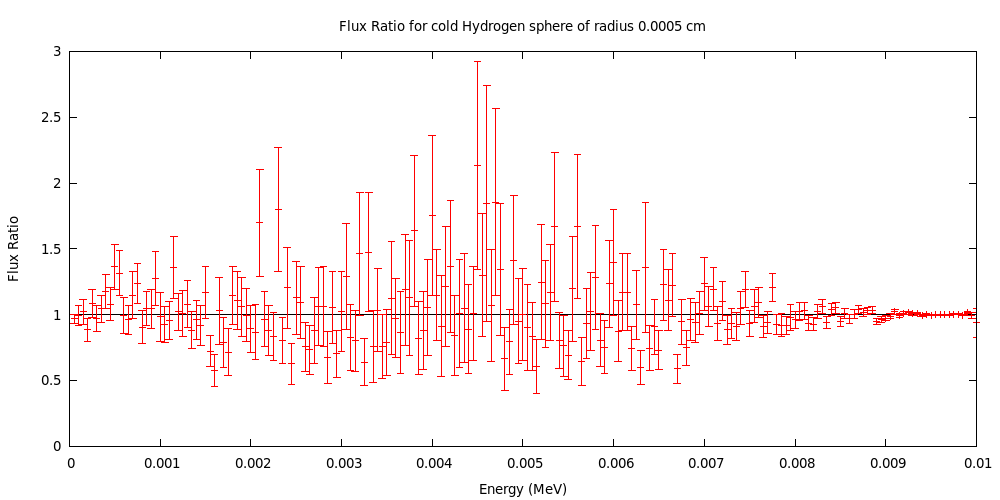
\includegraphics[width = 0.9\textwidth]{./Sphere1.png}
  \end{figure}


\end{frame}

%%----------------------------------------------------------------------------%%
\begin{frame}{Results}

  \begin{figure}
     \centering
     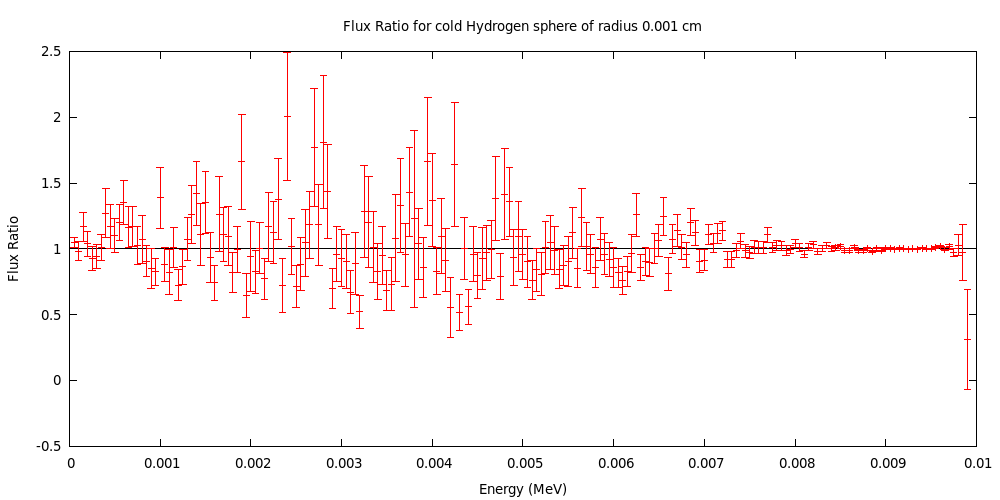
\includegraphics[width = 0.9\textwidth]{./Sphere2.png}
  \end{figure}


\end{frame}

%%----------------------------------------------------------------------------%%
\begin{frame}{Results}

  \begin{figure}
     \centering
     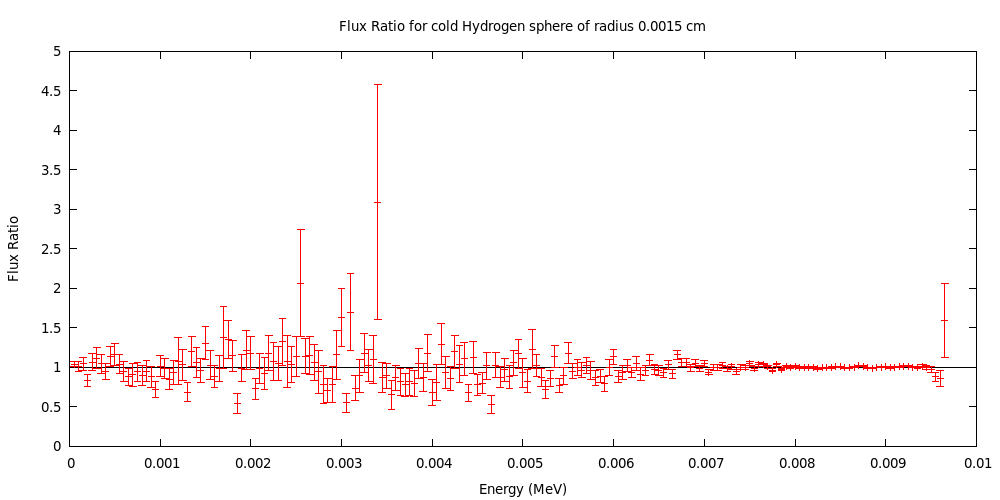
\includegraphics[width = 0.9\textwidth]{./Sphere3.png}
  \end{figure}


\end{frame}

%%----------------------------------------------------------------------------%%
\begin{frame}{Results}

  \begin{figure}
     \centering
     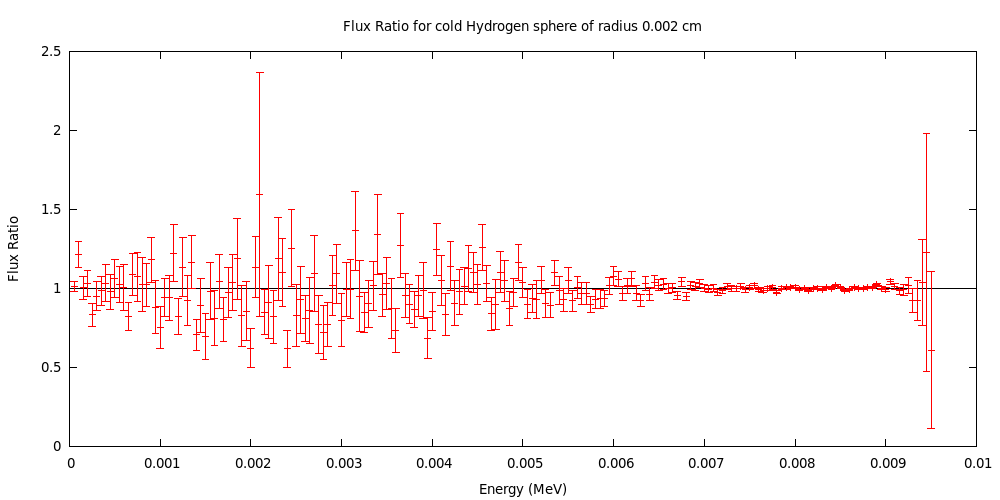
\includegraphics[width = 0.9\textwidth]{./Sphere4.png}
  \end{figure}


\end{frame}

%%----------------------------------------------------------------------------%%
\begin{frame}{Results}

  \begin{figure}
     \centering
     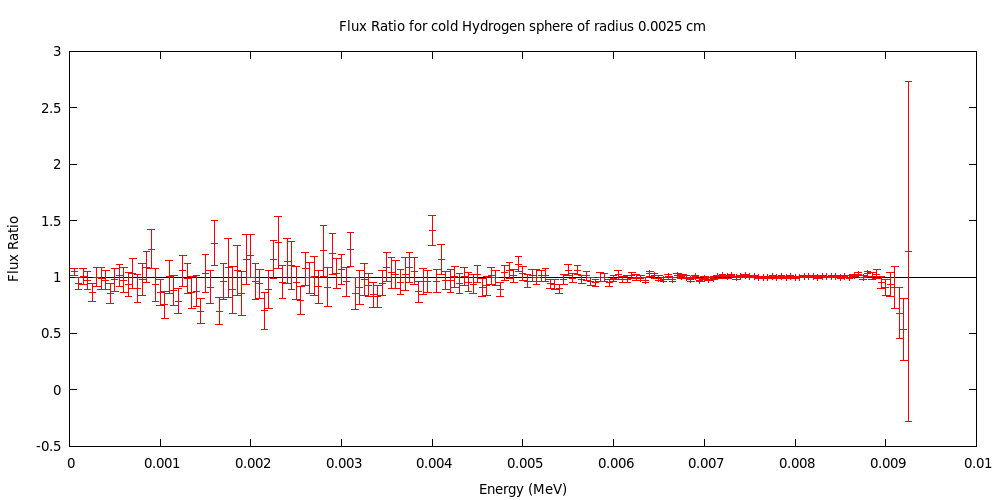
\includegraphics[width = 0.9\textwidth]{./Sphere5.png}
  \end{figure}


\end{frame}


%%----------------------------------------------------------------------------%%
\begin{frame}{Conclusions}
 
    \begin{itemize}
      \item The agreement is slightly below the $3~\sigma$ rule.
      
      \item There appears to be a tail off in the upper energy bins.
       
      \item Further testing is planned to evaluate the the single scattered spectrum.
  
      \item FRENSIE code currently runs 100x slower than MCNP6 for a simple geometry.
      
      \item Modifications need to be made to speed up transport in DAG geometry by reducing the number of ray firings.
      
      \item Implementation of Root's combinational geometry would also speed up geometry transport.
       
    \end{itemize}
\end{frame}

%%----------------------------------------------------------------------------%%
\begin{frame}{Possible Adjoint Methods}
  \begin{block}{Hybrid Multigroup/Continuous-Energy BFP}
 
    \begin{itemize}
      \item The same basic multigroup cross-section data can be used for forward and adjoint calculations. 
       
      \item The adjoint transport model is nearly identical to the forward making implementation easy.
    \end{itemize}
  \end{block}
  
  \begin{block}{Generalized Particle for Adjoint Transport}
    \begin{itemize}
        \item The CSDA is used with Moli\`{e}re's multiple scattering theory.
       
         \item No secondary particles are produced. One particle enters an event and one leaves.
    \end{itemize}
  \end{block}


\end{frame}


\end{document}
